\documentclass[handout]{beamer}
%\documentclass[presentation]{beamer}

\usecolortheme{Imperial}
 
\usepackage[utf8]{inputenc}
\usepackage[UKenglish]{babel}
\usepackage{booktabs}
\usepackage{caption}
\usepackage{subcaption}
\usepackage{graphicx}
\usepackage{amsmath, amssymb, amsthm, bm}
\usepackage{amsfonts}
\usepackage{amssymb}
\usepackage{epstopdf}
\usepackage{csquotes}
\usepackage{xcolor}
\usepackage{hyperref} 
\hypersetup{
    colorlinks=true,
    linkcolor=imperialblue,
    filecolor=blue,      
    citecolor=blue,
    urlcolor=blue,
    pdfpagemode=FullScreen,
}
\usepackage{natbib}
\bibliographystyle{plainnat}

% complying UK date format, i.e. 1 January 2001
\usepackage{datetime}
\let\dateUKenglish\relax
\newdateformat{dateUKenglish}{\THEDAY~\monthname[\THEMONTH] \THEYEAR}

% \institute{\includegraphics[height=0.7cm]{./images/Imperial_1_Pantone_solid.eps}}
\institute{\includegraphics[height=0.7cm]{./images/Imperial_1_Pantone_solid.eps}}

% -----------------------------------------------------------------------------




%Information to be included in the title page:
\title{Forecasting Returns for High Frequency Cryptocurrency WebSocket Data}

\subtitle{MSci Thesis Presentation}

\author{Isaac Lee}

\date{\today}


\AtBeginSection[]{
  \begin{frame}
  \vfill
  \centering
  \begin{beamercolorbox}[sep=8pt,center,shadow=false,rounded=true]{title}
    \usebeamerfont{title}\Huge\insertsectionhead\par%
  \end{beamercolorbox}
  \vfill
  \end{frame}
}


\begin{document}
 
\frame{\titlepage}

\begin{frame}
	\frametitle{Contents}
    \begin{enumerate}
        \item Introduction
        \item Orderbook Data
        \item Modelling Objective
        \item Model Theory
        \item Orderbook Features
        \item Model Architectures
        \item Methodology
        \item Results
        \item Conclusions
    \end{enumerate}
\end{frame}

\section{Introduction}

\begin{frame}
    \frametitle{Summary}
     \begin{itemize}
        \item Predict high frequency returns
        \item Introduce novel dataset
        \item Explore results for different models, trading pairs and prediction horizons
    \end{itemize}
\end{frame}

\begin{frame}
    \frametitle{Centralized Markets}
     \begin{itemize}
    \item Centralized vs. Decentralized
    \item Advantage: better regulation
    \item Disadvantage: must trust a third party
\end{itemize}
    
\end{frame}

\begin{frame}
    \frametitle{The Orderbook}
     \begin{itemize}
    \item Used to organize buying and selling activity
    \item Different order types, limit vs. market
    \item Snapshot of supply and demand
    \item Supply and demand drives price, {\color{blue}\cite{MANKIW2014}}
\end{itemize}
\end{frame}

\begin{frame}
    \frametitle{Simplified Orderbook Visualization}
    \begin{figure}[htpb]
        \centering
        \includegraphics[width=0.4\textwidth]{./images/orderbook.pdf}
        \caption{A simplified visualization of a limit orderbook.}
    \end{figure}
\end{frame}

\begin{frame}
    \frametitle{Related Works}
     \begin{itemize}
         \item Early methods were parametric, e.g. linear regressions, {\color{blue}\cite{CAO2009}}, or Hawkes processes, {\color{blue}\cite{HAWKES2013}}
        \item Explosion in popularity of deep learning
        \item DeepLOB, {\color{blue}\cite{ZHANG2019}}, DeepOF, {\color{blue}\cite{KOLM2023}}, DeepVOL, {\color{blue}\cite{LUCCHESE2024}}
        \item Relatively few papers for crypto data
        \item {\color{blue}\cite{AKYILDIRIM2023}} use traditional ML, {\color{blue}\cite{SHIN2021}} use LSTM models for Bitcoin futures prediction
        \item Both for longer time horizons of minutes, hours, days
    \end{itemize}
\end{frame}

\begin{frame}
    \frametitle{Contribution}
     \begin{itemize}
    \item Application to novel cryptocurrency data.
    \item Prediction horizons ranging from $\approx 500$ milliseconds to $\approx 20$ seconds for Binance perpetual futures limit orderbook WebSocket data
    \item Previous similar literature, {\color{blue}\cite{ZHANG2019}}, {\color{blue}\cite{KOLM2023}}, {\color{blue}\cite{LUCCHESE2024}}, was for NASDAQ data
    \item Also the use of XGBoost, {\color{blue}\cite{XGBOOST2016}}, for high frequency orderbook modelling. 
    \end{itemize}
    
\end{frame}

\section{Orderbook Data}
\begin{frame}
    \frametitle{Data Source}
     \begin{itemize}
        \item Binance, worlds largest centralized cryptocurrency exchange
        \item WebSocket, {\color{blue}\cite{WEBSOCKET2011}}, API endpoint:  \url{wss://fstream.binance.com/ws/{trading pair}@depth{L}@100ms}
        \item Logged to SQL database on AWS instance
        \item Data ranges from 2024-02-05 13:07:53.664 to 2024-02-25 11:18:50.866
        \item Between 11 to 13 million rows of data per trading pair
        \item Trading pairs: BTCUSDT, ETHUSDT, MATICUSDT, SOLUSDT
    \end{itemize}
    
\end{frame}

\begin{frame}
    \frametitle{Example Data}
    \begin{table}[ht]
    \centering
    \resizebox{0.99\textwidth}{!}{
        \begin{tabular}{llllllllllllll}
        \toprule
        Row & timestamp & ask\_price\_1 & ... & ask\_price\_10 & bid\_price\_1 & ... & bid\_price\_10 & ask\_qty\_1 & ... & ask\_qty\_10 & bid\_qty\_1 & ... & bid\_qty\_10 \\
        \midrule
        0 & 1707138494390 & 0.7877 & ... & 0.7886 & 0.7876 & ... & 0.7867 & 9368.0 & ... & 58006.0 & 15095.0 & ... & 44990.0 \\
        1 & 1707138494515 & 0.7877 & ... & 0.7886 & 0.7876 & ... & 0.7867 & 9367.0 & ... & 58006.0 & 15095.0 & ... & 84785.0 \\
        2 & 1707138494760 & 0.7877 & ... & 0.7886 & 0.7876 & ... & 0.7867 & 9367.0 & ... & 58006.0 & 15095.0 & ... & 44990.0 \\
        3 & 1707138494881 & 0.7877 & ... & 0.7886 & 0.7876 & ... & 0.7867 & 9367.0 & ... & 58006.0 & 15095.0 & ... & 44990.0 \\
        4 & 1707138495248 & 0.7877 & ... & 0.7886 & 0.7876 & ... & 0.7867 & 9356.0 & ... & 58006.0 & 15099.0 & ... & 44990.0 \\
        \vdots & \vdots & \vdots & \vdots & \vdots & \vdots & \vdots & \vdots & \vdots & \vdots & \vdots & \vdots & \vdots & \vdots \\
        11294483 & 1708857980137 & 0.9726 & ... & 0.9735 & 0.9725 & ... & 0.9716 & 16199.0 & ... & 64495.0 & 20555.0 & ... & 37554.0 \\
        11294484 & 1708857980246 & 0.9726 & ... & 0.9735 & 0.9725 & ... & 0.9716 & 16199.0 & ... & 61163.0 & 19527.0 & ... & 37554.0 \\
        11294485 & 1708857980360 & 0.9726 & ... & 0.9735 & 0.9725 & ... & 0.9716 & 20199.0 & ... & 61163.0 & 19527.0 & ... & 37554.0 \\
        11294486 & 1708857980494 & 0.9726 & ... & 0.9735 & 0.9725 & ... & 0.9716 & 21610.0 & ... & 61163.0 & 19577.0 & ... & 37554.0 \\
        11294487 & 1708857980602 & 0.9726 & ... & 0.9735 & 0.9725 & ... & 0.9716 & 22992.0 & ... & 61163.0 & 18401.0 & ... & 37554.0 \\
        \bottomrule
        \end{tabular}
    }
    \caption{Example data for MATICUSDT.}
    \label{table:websocket}
    \end{table}
\end{frame}



\begin{frame}
    \frametitle{Data Irregularities}
        \begin{table}[ht]
            \resizebox{\textwidth}{!}{
                \begin{tabular}{lrrrr}
                \toprule
                 & BTCUSDT $\Delta t$ ms & ETHUSDT $\Delta t$ ms & MATICUSDT $\Delta t$ ms & SOLUSDT $\Delta t$ ms \\
                \midrule
                count & 12891080 & 13612890 & 11294487 & 13334051 \\
                median & 116 & 114 & 122 & 115 \\
                mean & 133 & 126 & 152 & 129 \\
                std & 50& 41& 82& 47\\
                min & 3 & 3 & 3 & 3 \\
                25\% & 107 & 105 & 108 & 107 \\
                50\% & 116 & 114 & 122 & 115 \\
                75\% & 142 & 133 & 162 & 135 \\
                max & 61604 & 61862 & 61697 & 61815 \\
                \bottomrule
                \end{tabular}
            }

            \caption{Summary statistics for the time difference between observations in ms, $\Delta t$ ms, for each trading pair.}
            \label{timedelta_table}
        \end{table}
\end{frame}

\begin{frame}
    \frametitle{Orderbook Shape}
    \begin{figure}[ht]
        \centering
        \includegraphics[width=1.0\textwidth]{./images/shapes_1.pdf}
        \caption{Average orderbook shape for BTCUSDT and ETHUSDT.}
        \label{shape1}
    \end{figure}
\end{frame}

\begin{frame}
    \frametitle{Orderbook Shape}
    \begin{figure}[ht]
        \centering
        \includegraphics[width=1.0\textwidth]{./images/shapes_2.pdf}
        \caption{Average orderbook shape for MATICUSDT and SOLUSDT.}
        \label{shape2}
    \end{figure}
\end{frame}

\section{Modelling Objective}
\begin{frame}
    \frametitle{The Modelling Objective}
     \begin{itemize}
        \item Aim: predict direction of future smoothed mid-price
        \item Three class classification problem
    \end{itemize}
    
\end{frame}

\begin{frame}
    \frametitle{Smoothed Returns}
    Introduced in in {\color{blue}\cite{AVRAAM2017}}. Define the quantites:
        \begin{align}
            m_{-}(t) &:= \frac{1}{k} \sum_{i=0}^{k} p_0(t-i) \\
            m_{+}(t) &:= \frac{1}{k} \sum_{i=1}^{k} p_0(t+i) \\
            \ell(t) &:= \frac{m_{+}(t) - m_{-}(t)}{m_{-}(t)}
            \label{smoothed_returns}
        \end{align}
         \begin{itemize}
    \item $m_{-}(t)$/$m_{+}(t)$: average mid-price for the previous (inclusive)/next $k$ observations
\end{itemize}
\end{frame}

\begin{frame}
    \frametitle{Discretizing Smoothed Returns}
    Convert to a classification problem by discretizing returns:
    \begin{equation}
        y(t) = \begin{cases} \label{desc}
            +1  & \text{ if } \ell(t) \in (\epsilon, \infty) \\
            0  & \text{ if } \ell(t) \in [-\epsilon, \epsilon] \\
           -1  & \text{ if } \ell(t) \in  (-\infty, -\epsilon)
       \end{cases}
    \end{equation}
    Choice of $\epsilon$ discussed later.
\end{frame}


\begin{frame}
    \frametitle{Example Labelled Data}
        \begin{figure}[ht]
            \centering
            \includegraphics[width=1.0\textwidth]{./images/example_labels.pdf}
            \caption{An example BTCUSDT mid-price sample, coloured according to class label.}
            \label{fig:example_mid_price_labelling}
        \end{figure}
\end{frame}

\section{Model Theory}

\begin{frame}
    \frametitle{Logistic Regression}
     \begin{itemize}
        \item Introduced in {\color{blue}\cite{COX1958}}.
        \item Key idea: map the output of a linear model onto the interval [0, 1] using the logistic function:
            \begin{equation}
               \sigma(x) = \frac{1}{1 + \exp(-x)} 
            \end{equation}
        \item Treat these values as probabilities and select the class with the highest probability.
    \end{itemize}
    
\end{frame}

\begin{frame}
    \frametitle{Decision Trees}
     \begin{itemize}
        \item Optimal data partitioning using a tree datastructure
        \item Tree is built iteratively by selecting the best feature and threshold to split on at each node
        \item Greedy approach
        \item For classification, class label is the mode of the training samples in the leaf node
    \end{itemize}
    
\end{frame}

\begin{frame}
    \frametitle{Example Decision Tree}
        \begin{figure}[ht]
            \centering
            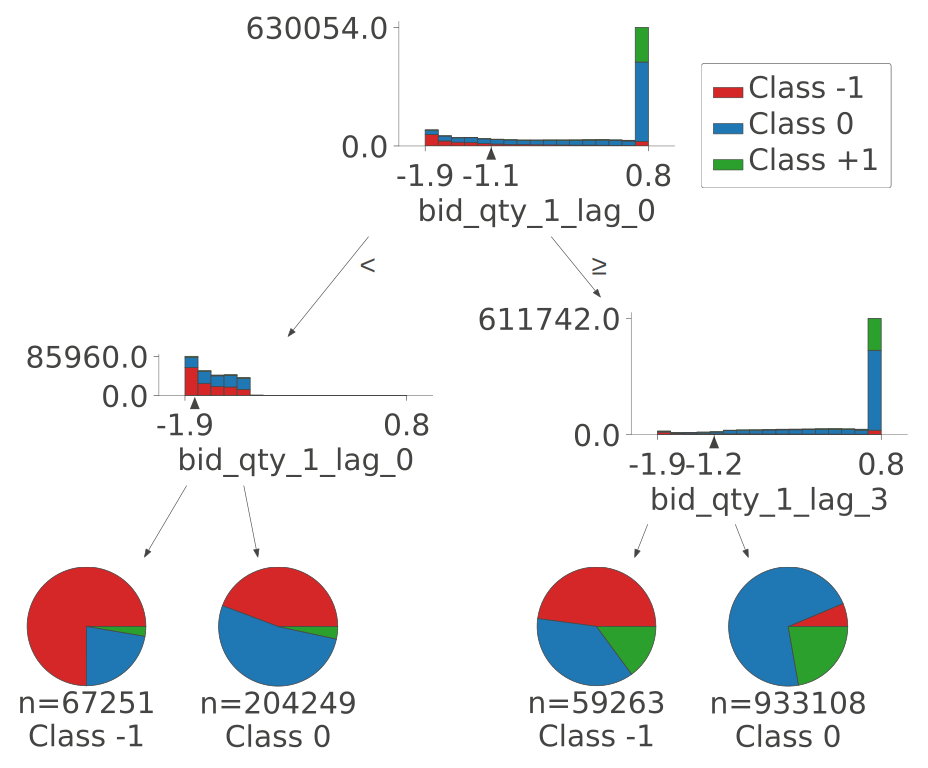
\includegraphics[width=0.6\textwidth]{./images/xgb_viz.pdf}
            \caption{A visualization of a single decision tree.}
            \label{fig:weaklearner}
        \end{figure}
\end{frame}

\begin{frame}
    \frametitle{Boosting and Boosted Decision Trees}
     \begin{itemize}
         \item Simple decision trees have high variance, leading to overfitting
         \item \textit{Boosting}, {\color{blue}\cite{HASTIE2001}}, is an ensemble method used to solve this problem
        \item Basic idea: iteratively train many \textit{weak learners} and then combine their predictions to produce a single, more robust prediction. 
        \item Boosting lowers the model bias, whilst keeping variance low.
    \end{itemize}
\end{frame}

\begin{frame}
    \frametitle{Neural Networks}
     \begin{itemize}
         \item Most famous example, the MLP, {\color{blue}\cite{RUMELHART1986}}.
        \item Affine and non-linear projections:
            \begin{equation*}
                \begin{aligned}
                    f_i(x; W_i, b_i) &:= \sigma_i(W_i x + b_i) \\
                    f(x; W_1, W_2, ..., W_N, b_1, b_2, ..., b_N) &:= f_N \circ f_{N-1} \circ ... \circ f_2 \circ f_1(x)
                \end{aligned}
            \end{equation*}
        \item {\color{blue}\cite{HORNIK1989}} shows, they are \textit{universal function approximators}
        \end{itemize}
\end{frame}

\begin{frame}
    \frametitle{Neural Networks}
     \begin{itemize}
     \item Loss function:
        \begin{equation}
           \mathcal{L} (\theta; x, y) := \frac{1}{n} \sum_{i=1}^{n} \ell(f(x_i; \theta), y_i)
        \end{equation}
    \item Gradient descent via \textit{backpropagation}, {\color{blue}\cite{RUMELHART1986}}:
        \begin{equation}
            \theta^{(t+1)} \gets \theta^{(t)} - \eta \nabla_\theta \mathcal{L}(\theta^{(t)})
        \end{equation}
    \item In practice non-convex local minima, so other methods e.g. \textit{stochastic gradient descent}, {\color{blue}\cite{ROBBINS1951}}, with \textit{momentum}, used.
\end{itemize}
\end{frame}

\begin{frame}
    \frametitle{Convolutional Neural Networks}
     \begin{itemize}
         \item Introduced in {\color{blue}\cite{LECUN1998}}
        \item Specialized class of NNs designed for processing structured grid data, such as images.
        \item Key advantages: local receptive fields, shared weights and spatial subsampling, {\color{blue}\cite{ABRAMS2017}}.
        \item Convolutional layer applies a convolution operation across previous layer:
            \begin{equation}
                \begin{aligned}
                    h_{ij} &= \sigma\left((W * x)_{ij} + b\right) \\
                    (W * x)_{ij} &:= \sum_{m=-k}^{k}\sum_{n=-k}^{k} W_{mn} x_{i-m, j-n}
                \end{aligned}
            \end{equation}
    \end{itemize} 
\end{frame}

\begin{frame}
    \frametitle{Convolution Visualized}
    \begin{figure}[htpb]
        \centering
        \includegraphics[width=0.8\textwidth]{./images/conv.png}
        \caption{Example convolutional fitler applied to a 2D array. Image source: {\color{blue}\cite{PODAREANU2019}}.}
    \end{figure}
    
\end{frame}

\begin{frame}
    \frametitle{Recurrent Neural Networks}
     \begin{itemize}

         \item RNNs are NNs that take in sequences of input iteratively.
        \item At each iteration: take in input and previous hidden state, update hidden state then output
        \item Famous example, the Jordan RNN, {\color{blue}\cite{JORDAN1997}}:
            \begin{equation}
                \begin{aligned}
                    h_t &= \sigma_h(W_h x_t + U_h y_{t-1} + b_h)  \\
                    y_t &= \sigma_y(W_y h_t + b_y)
                \end{aligned}
            \end{equation}
    \end{itemize}
    
\end{frame}

\begin{frame}
    \frametitle{Recurrent Neural Networks}
\begin{figure}[htpb]
    \centering
    \includegraphics[width=0.8\textwidth]{./images/RNN.png}
    \caption{A visualization of an RNN. Image source: {\color{blue}\cite{RNNIMAGE2024}}}
\end{figure}
    
\end{frame}

\begin{frame}
    \frametitle{Long Short-Term Memory}
     \begin{itemize}
         \item Vanilla RNNs suffer from \textit{vanishing gradients}, {\color{blue}\cite{PASCANU2013}}
         \item The LSTM, {\color{blue}\cite{HOCHREITER1997}} was devised to address this
         \item Main ideas: input gate, output gate, forget gate and cell
        \item Cell learns information and other gates regulate flow of information to the cell
        \item A modification of an RNN with more hidden state for greater control of what information is learnt 
    \end{itemize}
\end{frame}

\begin{frame}
    \frametitle{Long Short-Term Memory}
    \begin{equation}
        \begin{aligned}
            f_t &= \sigma_g(W_f x_t + U_f h_{t-1} + b_f) \\
            i_t &= \sigma_g(W_i x_t + U_i h_{t-1} + b_i) \\
            o_t &= \sigma_g(W_o x_t + U_o h_{t-1} + b_o) \\
            \tilde{c}_t &= \sigma_c(W_c x_t + U_c h_{t-1} + b_c) \\
                    c_t &= f_t \odot c_{t-1} + i_t \odot \tilde{c}_t \\
            h_t &= o_t \odot \sigma_h(c_t)
        \end{aligned}
    \end{equation}
    where $\odot$ denotes the element-wise product. {\color{blue}\cite{HOCHREITER1997}}.
\end{frame}

\section{Orderbook Features}
\begin{frame}
    \frametitle{The Raw Limit Orderbook Representation}
    {\color{blue}\cite{ZHANG2019}} use the raw orderbook data for their model input i.e. $\bm{x}_t$ takes the form:
    \begin{equation}
        \bm{x}_t = [p_{t, \ell}^A, q_{t, \ell}^A, p_{t, \ell}^B, q_{t, \ell}^B]_{\ell=1}^{L} \in \mathbb{R}^{4L}
    \end{equation}
\end{frame}

\begin{frame}
    \frametitle{The Orderflow Representation}
    Orderflow is a stationary transformation of the the raw orderbook data introduced in {\color{blue}\cite{CONT2013}}.
    Define the contribution of the $n^\text{th}$ event at level $\ell$ on the (A)sk/(B)id side as: 
    \begin{align}
        e_{t,\ell}^{A} &:=  I_{\{ p_{n, \ell}^A \leq p_{n-1,\ell}^A \}} q_{n}^A - I_{\{ p_{n, \ell}^A \geq p_{n-1, \ell}^A \}} q_{n-1, \ell}^A \\
        e_{t, \ell}^{B} &:= I_{\{ p_{n, \ell}^B \geq p_{n-1, \ell}^B \}} q_{n, \ell}^B - I_{\{ p_{n, \ell}^B \leq p_{n-1, \ell}^B \}} q_{n-1, \ell}^B
    \end{align}
    Then we define the Orderflow feature vector as:
    \begin{equation}
        \bm{x}_t := [e_{t, \ell}^{A}, e_{t, \ell}^{B}]_{\ell=1}^L \in \mathbb{R}^{2L} \label{OF_feature_vector}
    \end{equation}
\end{frame}

\begin{frame}
    \frametitle{lrLOB \& lrOF}
     \begin{itemize}
        \item For LOB/OF features concatenate with lagged features:
            \begin{equation}
                \bm{x}^{AR}_t = [\bm{x}_t; \bm{x}_{t-1}; \bm{x}_{t-2}; \cdots; \bm{x}_{T-1}] \in  \mathbb{R}^{dT}\label{AR_features}
            \end{equation}
        \item lrLOB: logistic regression model with raw limit orderbook AR features
        \item lrOF: logistic regression model with orderflow AR features
        \item $T := 10$ (memory constraints)
    \end{itemize}
    
\end{frame}

\begin{frame}
    \frametitle{xgbLOB \& xgbOF}
     \begin{itemize}
         \item XGBoost first introduced in {\color{blue}\cite{XGBOOST2016}}
        \item Efficient implementation of Boosted Decision Trees
        \item xgbLOB: XGBoost model with raw limit orderbook AR features
        \item xgbOF: XGBoost model with orderflow AR features
        \item $T := \min(20, k)$ (memory constraints)
    \end{itemize}
    
\end{frame}

\begin{frame}
    \frametitle{xgbLOB \& xgbOF Hyperparameters}
     \begin{itemize}
        \item \textbf{max depth} = 10. The max depth of each weak learner tree.
        \item \textbf{eta} = 0.1. Step size shrinkage used in update to prevent overfitting. After each boosting step, we can directly get the weights of new features, and eta shrinks the feature weights to make the boosting process more conservative.
        \item \textbf{data subsample ratio} = 0.8. The proportion of the training data that each weak learner can use.
        \item \textbf{column subsample ratio} = 0.8. The proportion of the features available when performing splits.
        \item \textbf{evaluation metric} = Multiclass classification error rate. The metric used during the boosting algorithm to determine weights.
    \end{itemize}
\end{frame}


\begin{frame}
    \frametitle{DeepLOB}
     \begin{itemize}
         \item First introduced in {\color{blue}\cite{ZHANG2019}}
        \item CNN-LSTM architecture
        \item Input $X_t \in \mathbb{R}^{T \times 4L}, X_t :=$
            \tiny
        \begin{equation}
            \begingroup
            \setlength\arraycolsep{1pt}
            \begin{bmatrix}
            p_{t-T, 1}^A & q_{t-T, 1}^A & p_{t-T, 1}^B &  q_{t-T, 1}^B &  \cdots & p_{t-T, L}^A &  q_{t-T, L}^A & p_{t-T, L}^B & q_{t-T, L}^B\\
            p_{t-(T-1), 1}^A & q_{t-(T-1), 1}^A & p_{t-(T-1), 1}^B &  q_{t-(T-1), 1}^B &  \cdots & p_{t-(T-1), L}^A &  q_{t-(T-1), L}^A & p_{t-(T-1), L}^B & q_{t-(T-1), L}^B\\
            \vdots & \vdots & \vdots & \vdots & \ddots & \vdots & \vdots& \vdots & \vdots\\
            p_{t-1, 1}^A & q_{t-1, 1}^A & p_{t-1, 1}^B &  q_{t-1, 1}^B &  \cdots & p_{t-1, L}^A &  q_{t-1, L}^A & p_{t-1, L}^B & q_{t-1, L}^B\\
            p_{t, 1}^A & q_{t, 1}^A & p_{t, 1}^B &  q_{t, 1}^B &  \cdots & p_{t, L}^A &  q_{t, L}^A & p_{t, L}^B & q_{t, L}^B\\
            \end{bmatrix}
            \endgroup
        \end{equation}
    \end{itemize}
    
\end{frame}

\begin{frame}
    \frametitle{DeepLOB Schematic}
    \begin{figure}[htpb]
        \centering
        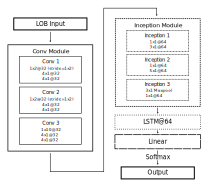
\includegraphics[width=0.6\textwidth]{./images/deepLOB_architecture.pdf}
        \caption{DeepLOB model schematic. Note: $1\times 2 @32$ means 32 $1 \times 2$ convolutional filters.}
    \end{figure}
\end{frame}

\begin{frame}
    \frametitle{DeepLOB Modules}
     \begin{itemize}
        \item \textbf{Convolutional Module}
             \begin{itemize}
                \item Conv 1 aggregates price and volume information for each level for each side
                \item Conv 2 aggregates information across side for each level
                \item Conv 3 aggregates information across the whole orderbook
            \end{itemize}
        \item \textbf{Inception Module}
             \begin{itemize}
                 \item Increases dimensionality and simulates moving averages
                 \item Key idea: \textit{Network-In-Network}, {\color{blue}\cite{MIN2014}}
            \end{itemize}
        \item \textbf{LSTM Module}
             \begin{itemize}
                 \item Captures long term dependencies from inception output
            \end{itemize}
    \end{itemize}
\end{frame}


\begin{frame}
    \frametitle{DeepOF}
     \begin{itemize}
         \item Introduced in {\color{blue}\cite{KOLM2023}}
        \item Modification of the DeepLOB architecture: uses orderflow input instead of raw orderbook
        \item Input:
            \small
            \begin{equation*}
                X_{t} := \begin{bmatrix}
                e_{t-T, 1}^A & e_{t-T, 1}^B &   \cdots & e_{t-T, L}^A & e_{t-T, L}^B \\
                e_{t-(T-1), 1}^A & e_{t-(T-1), 1}^B &   \cdots & e_{t-(T-1), L}^A & e_{t-(T-1), L}^B \\
                \vdots & \vdots & \ddots & \vdots & \vdots \\
                e_{t-1, 1}^A & e_{t-1, 1}^B &  \cdots & e_{t-1, L}^A & e_{t-1, L}^B \\
                e_{t, 1}^A & e_{t, 1}^B &  \cdots & e_{t, L}^A & e_{t, L}^B \\
                \end{bmatrix} \in \mathbb{R}^{T \times 2L}
                \label{DeepLOB_input}
            \end{equation*}
    \end{itemize}
\end{frame}

\section{Methodology}
\begin{frame}
    \frametitle{Sliding Window Setup}
    \begin{figure}[htpb]
        \centering
        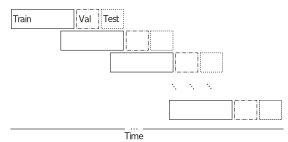
\includegraphics[width=0.9\textwidth]{./images/sliding_window.pdf}
        \caption{Train-val-test windows visualization. Note: train windows are 48 hours and val and test are 24 hours.}
    \end{figure}
\end{frame}

\begin{frame}
    \frametitle{Data Normalization}
     \begin{itemize}
        \item Calculate sample mean and standard deviation for each training window
        \item Scale train, val and test windows with:
            \begin{equation*}
                \begin{aligned}
                    \tilde{X}_{\text{train}} &= \frac{X_{\text{train}} - \mu_{\text{train}}}{\sigma_{\text{train}}} \\
                    \tilde{X}_{\text{val}} &= \frac{X_{\text{val}} - \mu_{\text{train}}}{\sigma_{\text{train}}} \\
                    \tilde{X}_{\text{test}} &= \frac{X_{\text{train}} - \mu_{\text{test}}}{\sigma_{\text{train}}}
                \end{aligned}
            \end{equation*}
    \end{itemize}
    
\end{frame}

\begin{frame}
    \frametitle{Choice of Label Discretization Parameter}
     \begin{itemize}
         \item Following {\color{blue}\cite{LUCCHESE2024}}, set discretization parameter, $\epsilon$, so that classes are balanced
        \item For prediction horizon $k$, window $w$:
        \begin{equation}
            \epsilon := \epsilon_{k, w} := \frac{|\hat{F}_{k, w}^{-1}(\frac{1}{3})| + \hat{F}_{k, w}^{-1}(\frac{2}{3})}{2}
        \end{equation}
    \end{itemize}
\end{frame}

\begin{frame}
    \frametitle{Model Training}
     \begin{itemize}
         \item DeepLOB and DeepOF trained with PyTorch {\color{blue}\cite{PYTORCH2017}}
        \item Hardware: Nvidia RTX 3060 12GB, 64GB memory, 14 core 20 thread Intel i5 13600K
        \item Optimizer: ADAM, {\color{blue}\cite{ADAM2017}}
        \item Loss: Cross Entropy Loss
        \item Trained until validation loss plateaued
    \end{itemize}
    
\end{frame}

\section{Results}
\begin{frame}
    \frametitle{Classification Metrics}
     \footnotesize
     \begin{itemize}
        \item Precision for class $ c $ is:
            \begin{equation}
            \text{Precision}_c := \frac{\text{TP}_c}{\text{TP}_c + \text{FP}_c}
            \end{equation}
        \textit{``Out of all the times that we guessed class $c$, how many times were we correct?''}
        \item Recall for class $c$ is:
            \begin{equation}
            \text{Recall}_c := \frac{\text{TP}_c}{\text{TP}_c + \text{FN}_c}
            \end{equation}
            \textit{``Out of all the times the true class was $c$, how many times did we predict it correctly?''}
        \item F1-score for class $ c $ is harmonic mean of precision and recall:
            \begin{equation}
            \text{F1-score}_c := 2 \cdot \frac{\text{Precision}_c \cdot \text{Recall}_c}{\text{Precision}_c + \text{Recall}_c}
            \end{equation}
    \end{itemize}
\end{frame}

\begin{frame}
    \frametitle{Macro-Averages Averaged Across Windows, $k=4$}
    \begin{table}[H]
    \resizebox{0.99\textwidth}{!}{
    \begin{tabular}{llllll}
    \toprule
    accuracy & precision & recall & f1-score & support & model \\
    \midrule
    \textbf{0.87}(0.03) & \textbf{0.91}(0.03) & \textbf{0.74}(0.01) & \textbf{0.80}(0.01) & 647295(30003) & \textbf{xgbOF} \\
    0.79(0.04) & 0.75(0.05) & 0.68(0.02) & 0.70(0.01) & 647295(30003) & xgbLOB \\
    0.84(0.04) & 0.87(0.02) & 0.70(0.01) & 0.76(0.01) & 647289(30003) & lrOF \\
    0.69(0.07) & 0.66(0.08) & 0.60(0.07) & 0.59(0.06) & 647289(30003) & lrLOB \\
    0.86(0.03) & 0.88(0.03) & \textbf{0.74}(0.01) & 0.79(0.0) & 647199(30003) & deepOF \\
    0.75(0.2) & 0.73(0.22) & 0.70(0.04) & 0.69(0.17) & 647199(30003) & deepLOB \\
    \bottomrule
    \end{tabular}
    }
    \caption{Mean macro averaged BTCUSDT test set classification results across windows for $\bm{k=4}$. (Standard deviations are given in parenthesis).}
    \label{macro_table_1}
    \end{table}
\end{frame}

\begin{frame}
    \frametitle{Macro-Averages Averaged Across Windows, $k=10$}
        \begin{table}[H]
        \resizebox{0.99\textwidth}{!}{
        \begin{tabular}{llllll}
        \toprule
        accuracy & precision & recall & f1-score & support & model \\
        \midrule
        \textbf{0.80}(0.03) & \textbf{0.84}(0.04) & 0.75(0.01) & \textbf{0.78}(0.02) & 647289(30003) & \textbf{xgbOF} \\
        0.72(0.02) & 0.71(0.02) & 0.71(0.01) & 0.71(0.01) & 647289(30003) & xgbLOB \\
        0.76(0.04) & 0.81(0.03) & 0.72(0.01) & 0.74(0.02) & 647289(30003) & lrOF \\
        0.58(0.07) & 0.62(0.05) & 0.62(0.04) & 0.57(0.08) & 647289(30003) & lrLOB \\
        0.79(0.03) & 0.81(0.02) & \textbf{0.76}(0.01) & 0.77(0.01) & 647199(30003) & deepOF \\
        0.74(0.06) & 0.76(0.04) & 0.71(0.05) & 0.72(0.06) & 647199(30003) & deepLOB \\
        \bottomrule
        \end{tabular}
        }
        \caption{Mean macro averaged BTCUSDT test set classification results across windows for $\bm{k=10}$.}
        \label{macro_table_2}
        \end{table}
\end{frame}

\begin{frame}
    \frametitle{Macro-Averages Averaged Across Windows, $k=50$}
        \begin{table}[H]
        \resizebox{0.99\textwidth}{!}{
            \begin{tabular}{llllll}
            \toprule
            accuracy & precision & recall & f1-score & support & model \\
            \midrule
            0.64(0.04) & \textbf{0.65}(0.03) & 0.62(0.01) & 0.63(0.02) & 647279(30003) & xgbOF \\
            0.56(0.04) & 0.57(0.03) & 0.58(0.04) & 0.53(0.06) & 647279(30003) & xgbLOB \\
            0.57(0.05) & 0.62(0.03) & 0.55(0.0) & 0.55(0.02) & 647289(30003) & lrOF \\
            0.51(0.06) & 0.52(0.03) & 0.54(0.03) & 0.46(0.06) & 647289(30003) & lrLOB \\
            \textbf{0.66}(0.03) & \textbf{0.65}(0.02) & \textbf{0.65}(0.02) & \textbf{0.65}(0.02) & 647199(30003) & \textbf{deepOF} \\
            0.57(0.07) & 0.58(0.04) & 0.57(0.07) & 0.55(0.09) & 647199(30003) & deepLOB \\
            \bottomrule
            \end{tabular}
        }
        \caption{Mean macro averaged BTCUSDT test set classification results across windows for $\bm{k=50}$.}
        \label{macro_table_3}
        \end{table}
\end{frame}

\begin{frame}
    \frametitle{Macro-Averages Averaged Across Windows, $k=200$}
        \begin{table}[H]
        \resizebox{0.99\textwidth}{!}{
            \begin{tabular}{llllll}
            \toprule
            accuracy & precision & recall & f1-score & support & model \\
            \midrule
            0.52(0.04) & 0.53(0.03) & 0.50(0.01) & 0.51(0.01) & 647279(30003) & xgbOF \\
            0.46(0.04) & 0.45(0.02) & 0.48(0.02) & 0.40(0.04) & 647279(30003) & xgbLOB \\
            0.48(0.05) & 0.50(0.02) & 0.46(0.01) & 0.45(0.01) & 647289(30003) & lrOF \\
            0.44(0.05) & 0.45(0.04) & 0.47(0.03) & 0.39(0.04) & 647289(30003) & lrLOB \\
            \textbf{0.56}(0.03) & \textbf{0.56}(0.02) & \textbf{0.55}(0.02) & \textbf{0.55}(0.02) & 647199(30003) & \textbf{deepOF} \\
            0.49(0.05) & 0.48(0.04) & 0.49(0.06) & 0.47(0.05) & 647199(30003) & deepLOB \\
            \bottomrule
            \end{tabular}
        }
        \caption{Mean macro averaged BTCUSDT test set classification results across windows for $\bm{k=200}$.}
        \label{macro_table_4}
        \end{table}
\end{frame}

\begin{frame}
    \frametitle{BTCUSDT Window-Wise Macro Averages, $k=4$}
    \begin{figure}[htpb!]
        \centering
        \includegraphics[width=1.0\textwidth]{./images/BTCUSDT_macro_results_k=4.pdf}
        \caption{Comparing the macro averaged precision, recall and F1 score on the unseen test set for each window, for each trading pair, for $k=4$.}
        
    \end{figure}
\end{frame}

\begin{frame}
    \frametitle{ETHUSDT Window-Wise Macro Averages, $k=4$}
    \begin{figure}[htpb!]
        \centering
        \includegraphics[width=1.0\textwidth]{./images/ETHUSDT_macro_results_k=4.pdf}
        \caption{Comparing the macro averaged precision, recall and F1 score on the unseen test set for each window, for each trading pair, for $k=4$.}
        
    \end{figure}
\end{frame}

\begin{frame}
    \frametitle{MATICUSDT Window-Wise Macro Averages, $k=4$}
    \begin{figure}[htpb!]
        \centering
        \includegraphics[width=1.0\textwidth]{./images/MATICUSDT_macro_results_k=4.pdf}
        \caption{Comparing the macro averaged precision, recall and F1 score on the unseen test set for each window, for each trading pair, for $k=4$.}
        
    \end{figure}
\end{frame}

\begin{frame}
    \frametitle{SOLUSDT Window-Wise Macro Averages, $k=4$}
    \begin{figure}[htpb!]
        \centering
        \includegraphics[width=1.0\textwidth]{./images/SOLUSDT_macro_results_k=4.pdf}
        \caption{Comparing the macro averaged precision, recall and F1 score on the unseen test set for each window, for each trading pair, for $k=4$.}
        
    \end{figure}
\end{frame}


\begin{frame}
    \frametitle{BTCUSDT Window-Wise Macro Averages, $k=10$}
    \begin{figure}[htpb!]
        \centering
        \includegraphics[width=1.0\textwidth]{./images/BTCUSDT_macro_results_k=10.pdf}
        \caption{Comparing the macro averaged precision, recall and F1 score on the unseen test set for each window, for each trading pair, for $k=10$.}
        
    \end{figure}
\end{frame}

\begin{frame}
    \frametitle{ETHUSDT Window-Wise Macro Averages, $k=10$}
    \begin{figure}[htpb!]
        \centering
        \includegraphics[width=1.0\textwidth]{./images/ETHUSDT_macro_results_k=10.pdf}
        \caption{Comparing the macro averaged precision, recall and F1 score on the unseen test set for each window, for each trading pair, for $k=10$.}
        
    \end{figure}
\end{frame}

\begin{frame}
    \frametitle{MATICUSDT Window-Wise Macro Averages, $k=10$}
    \begin{figure}[htpb!]
        \centering
        \includegraphics[width=1.0\textwidth]{./images/MATICUSDT_macro_results_k=10.pdf}
        \caption{Comparing the macro averaged precision, recall and F1 score on the unseen test set for each window, for each trading pair, for $k=10$.}
        
    \end{figure}
\end{frame}

\begin{frame}
    \frametitle{SOLUSDT Window-Wise Macro Averages, $k=10$}
    \begin{figure}[htpb!]
        \centering
        \includegraphics[width=1.0\textwidth]{./images/SOLUSDT_macro_results_k=10.pdf}
        \caption{Comparing the macro averaged precision, recall and F1 score on the unseen test set for each window, for each trading pair, for $k=10$.}
        
    \end{figure}
\end{frame}

\begin{frame}
    \frametitle{BTCUSDT Window-Wise Macro Averages, $k=50$}
    \begin{figure}[htpb!]
        \centering
        \includegraphics[width=1.0\textwidth]{./images/BTCUSDT_macro_results_k=50.pdf}
        \caption{Comparing the macro averaged precision, recall and F1 score on the unseen test set for each window, for each trading pair, for $k=50$.}
        
    \end{figure}
\end{frame}

\begin{frame}
    \frametitle{ETHUSDT Window-Wise Macro Averages, $k=50$}
    \begin{figure}[htpb!]
        \centering
        \includegraphics[width=1.0\textwidth]{./images/ETHUSDT_macro_results_k=50.pdf}
        \caption{Comparing the macro averaged precision, recall and F1 score on the unseen test set for each window, for each trading pair, for $k=50$.}
        
    \end{figure}
\end{frame}

\begin{frame}
    \frametitle{MATICUSDT Window-Wise Macro Averages, $k=50$}
    \begin{figure}[htpb!]
        \centering
        \includegraphics[width=1.0\textwidth]{./images/MATICUSDT_macro_results_k=50.pdf}
        \caption{Comparing the macro averaged precision, recall and F1 score on the unseen test set for each window, for each trading pair, for $k=50$.}
        
    \end{figure}
\end{frame}

\begin{frame}
    \frametitle{SOLUSDT Window-Wise Macro Averages, $k=50$}
    \begin{figure}[htpb!]
        \centering
        \includegraphics[width=1.0\textwidth]{./images/SOLUSDT_macro_results_k=50.pdf}
        \caption{Comparing the macro averaged precision, recall and F1 score on the unseen test set for each window, for each trading pair, for $k=50$.}
        
    \end{figure}
\end{frame}

\begin{frame}
    \frametitle{BTCUSDT Window-Wise Macro Averages, $k=200$}
    \begin{figure}[htpb!]
        \centering
        \includegraphics[width=1.0\textwidth]{./images/BTCUSDT_macro_results_k=200.pdf}
        \caption{Comparing the macro averaged precision, recall and F1 score on the unseen test set for each window, for each trading pair, for $k=200$.}
        
    \end{figure}
\end{frame}

\begin{frame}
    \frametitle{ETHUSDT Window-Wise Macro Averages, $k=200$}
    \begin{figure}[htpb!]
        \centering
        \includegraphics[width=1.0\textwidth]{./images/ETHUSDT_macro_results_k=200.pdf}
        \caption{Comparing the macro averaged precision, recall and F1 score on the unseen test set for each window, for each trading pair, for $k=200$.}
        
    \end{figure}
\end{frame}

\begin{frame}
    \frametitle{MATICUSDT Window-Wise Macro Averages, $k=200$}
    \begin{figure}[htpb!]
        \centering
        \includegraphics[width=1.0\textwidth]{./images/MATICUSDT_macro_results_k=200.pdf}
        \caption{Comparing the macro averaged precision, recall and F1 score on the unseen test set for each window, for each trading pair, for $k=200$.}
        
    \end{figure}
\end{frame}

\begin{frame}
    \frametitle{SOLUSDT Window-Wise Macro Averages, $k=200$}
    \begin{figure}[htpb!]
        \centering
        \includegraphics[width=1.0\textwidth]{./images/SOLUSDT_macro_results_k=200.pdf}
        \caption{Comparing the macro averaged precision, recall and F1 score on the unseen test set for each window, for each trading pair, for $k=200$.}
        
    \end{figure}
\end{frame}

\begin{frame}
    \frametitle{xgbOF Confusion Matrices, BTCUSDT}
    \begin{figure}[htpb!]
        \centering
        \includegraphics[width=1.0\textwidth]{./images/BTCUSDT_xgbOF_confusion_matrices.pdf}
        \caption{BTCUSDT xgbOF confusion matrices. Note that counts are summed across windows.}
    \end{figure}
\end{frame}

\begin{frame}
    \frametitle{xgbLOB Confusion Matrices, BTCUSDT}
    \begin{figure}[htpb!]
        \centering
        \includegraphics[width=1.0\textwidth]{./images/BTCUSDT_xgbLOB_confusion_matrices.pdf}
        \caption{BTCUSDT xgbLOB confusion matrices. Note that counts are summed across windows.}
    \end{figure}
\end{frame}

\begin{frame}
    \frametitle{lrOF Confusion Matrices, BTCUSDT}
    \begin{figure}[htpb!]
        \centering
        \includegraphics[width=1.0\textwidth]{./images/BTCUSDT_lrOF_confusion_matrices.pdf}
        \caption{BTCUSDT lrOF confusion matrices. Note that counts are summed across windows.}
    \end{figure}
\end{frame}

\begin{frame}
    \frametitle{lrLOB Confusion Matrices, BTCUSDT}
    \begin{figure}[htpb!]
        \centering
        \includegraphics[width=1.0\textwidth]{./images/BTCUSDT_lrLOB_confusion_matrices.pdf}
        \caption{BTCUSDT lrLOB confusion matrices. Note that counts are summed across windows.}
    \end{figure}
\end{frame}


\begin{frame}
    \frametitle{deepOF Confusion Matrices, BTCUSDT}
    \begin{figure}[htpb!]
        \centering
        \includegraphics[width=1.0\textwidth]{./images/BTCUSDT_deepOF_confusion_matrices.pdf}
        \caption{BTCUSDT deepOF confusion matrices. Note that counts are summed across windows.}
    \end{figure}
\end{frame}

\begin{frame}
    \frametitle{deepLOB Confusion Matrices, BTCUSDT}
    \begin{figure}[htpb!]
        \centering
        \includegraphics[width=1.0\textwidth]{./images/BTCUSDT_deepLOB_confusion_matrices.pdf}
        \caption{BTCUSDT deepLOB confusion matrices. Note that counts are summed across windows.}
    \end{figure}
\end{frame}


\begin{frame}
    \frametitle{Top 10 LOB Feature Importances}
    \begin{figure}[htpb]
        \centering
        \includegraphics[width=1.0\textwidth]{./images/xgboost_LOB_BTCUSDT_top_10_feature_importances.pdf}
        \caption{Top 10 XGBoost LOB Feature Importances for BTCUSDT, measured by weight = number of times a feature was split on.}
    \end{figure}
\end{frame}

\begin{frame}
    \frametitle{Top 10 OF Feature Importances}
    \begin{figure}[htpb]
        \centering
        \includegraphics[width=1.0\textwidth]{./images/xgboost_OF_BTCUSDT_top_10_feature_importances.pdf}
        \caption{Top 10 XGBoost OF Feature Importances for BTCUSDT, measured by weight = number of times a feature was split on.}
    \end{figure}
\end{frame}

\begin{frame}
    \frametitle{Feature Ordering Recap}
     \begin{itemize}
        \item LOB features:
            \begin{equation*}
                \begin{aligned}
                    &[\text{ask}\_\text{price}\_\ell\_\text{lag}\_p, \text{ask}\_\text{qty}\_\ell\_\text{lag}\_p, \\
                    &\text{bid}\_\text{price}\_\ell\_\text{lag}\_p, \text{bid}\_\text{qty}\_\ell\_\text{lag}\_p]_{\ell = 1, ..., 10, p = 0, ..., T}
                \end{aligned}
            \end{equation*}
        \item OF features:
            \begin{equation*}
                [\text{ask}\_\text{orderflow}\_\ell\_\text{lag}\_p, \text{bid}\_\text{orderflow}\_\ell\_\text{lag}\_p]_{\ell = 1, ..., 10, p = 0, ..., T}
            \end{equation*}
        \item I.e. we first enumerate levels and then lags
    \end{itemize}
\end{frame}

\begin{frame}
    \frametitle{All non-zero LOB Feature Importances, $k=4, 10$}
        \begin{figure}[htpb!]
            \centering
            \includegraphics[width=1.0\textwidth]{./images/xgboost_LOB_BTCUSDT_all_feature_importances_1.pdf}
            \caption{All non-zero LOB feature importances for BTCUSDT, measured by weight = number of times a feature was split on.
            Note that the colors represent unique (feature type, lag) pairs, where feature type is either quantity or price and lag $\in \{0, ..., T\} $,
            e.g. the first color represents price features with lag 0.}
        \end{figure}
\end{frame}


\begin{frame}
    \frametitle{All non-zero LOB Feature Importances, $k=50, 200$}
        \begin{figure}[htpb!]
            \centering
            \includegraphics[width=1.0\textwidth]{./images/xgboost_LOB_BTCUSDT_all_feature_importances_1.pdf}
            \caption{All non-zero LOB feature importances for BTCUSDT, measured by weight = number of times a feature was split on.
            Note that the colors represent unique (feature type, lag) pairs, where feature type is either quantity or price and lag $\in \{0, ..., T\} $,
            e.g. the first color represents price features with lag 0.}
        \end{figure}
\end{frame}

\begin{frame}
    \frametitle{All non-zero OF Feature Importances, $k=4, 10$}
    \begin{figure}[htpb!]
        \centering
        \includegraphics[width=1.0\textwidth]{./images/xgboost_OF_BTCUSDT_all_feature_importances_1.pdf}
        \caption{All non-zero OF feature importances for BTCUSDT, measured by weight = number of times a feature was split on.
        Note that the colors represent unique lags, where lag $\in \{0, ..., T\} $. 
        E.g. the first color represents all features with lag 0.}
    \end{figure}
\end{frame}

\begin{frame}
    \frametitle{All non-zero OF Feature Importances, $k=50, 200$}
    \begin{figure}[htpb!]
        \centering
        \includegraphics[width=1.0\textwidth]{./images/xgboost_OF_BTCUSDT_all_feature_importances_2.pdf}
        \caption{All non-zero OF feature importances for BTCUSDT, measured by weight = number of times a feature was split on.
        Note that the colors represent unique lags, where lag $\in \{0, ..., T\} $. 
        E.g. the first color represents all features with lag 0.}
    \end{figure}
\end{frame}


\section{Conclusion}

\begin{frame}
    \frametitle{Conclusions}
     \begin{itemize}
        \item Precision of non-zero classes is perhaps most important for trading applications
        \item xgbOF is the winner for $k=4$ and $k=10$, with precision of $\approx 90\%$ for non-zero classes
        \item deepOF is the winner for $k=50$ and $k=200$ with non-zero class precision $\approx 60\%$
        \item Orderflow representation is far superior to raw orderbook representation
    \end{itemize}
    
\end{frame}

\begin{frame}
    \frametitle{Future Work}
     \begin{itemize}
         \item Compare models to those found in {\color{blue}\cite{ZHANG2019}}, {\color{blue}\cite{KOLM2023}}, {\color{blue}\cite{LUCCHESE2024}} when applied to their data
        \item Only considered 4 trading pairs, Binance has over 200
        \item Live data lends itself to \textit{online} modelling $\implies$ continuously test models
    \end{itemize}
    
\end{frame}

\begin{frame}[allowframebreaks]
        \frametitle{References}
        % \printbibliography
        \bibliography{bibliography.bib}
\end{frame}

 
\end{document}
